%\documentclass[english, 10pt, conference, letterpaper]{IEEEtran}
%\documentclass[english,10pt, draftclsnofoot, onecolumn]{IEEEtran}
\documentclass[english,10pt]{article}
%\usepackage[T1]{fontenc}
%\usepackage[latin9]{inputenc}
\usepackage[letterpaper]{geometry}
\geometry{verbose,tmargin=1cm,bmargin=2.5cm, lmargin = 2.5cm}
\usepackage{amsthm}
\usepackage{amsmath}
\usepackage{amssymb}
\usepackage{setspace}
\usepackage{graphicx}
\usepackage{color}
\usepackage{tabularx}
\usepackage{float}

\hyphenpenalty=0

\tolerance=1000000

\newcommand{\red}[1]{\begin{color}{red}{#1}\end{color}}
\newcommand{\MCL}[1]{\mathcal{#1}}
\newcommand{\BS}[1]{\boldsymbol{#1}}
\newcommand{\E}[0]{\mathbb{E}}



\newtheorem{theorem}{Theorem}
\newtheorem{proposition}{Proposition}
\newtheorem{corollary}{Corollary}

\makeatletter
\@ifundefined{date}{}{\date{}}
\makeatother

\usepackage{babel}
\begin{document}

\title{A comparison of wagering mechanisms by simulation}
\maketitle

\section{Mechanism}
	\begin{itemize}
	\item Competitive scoring rule with Brier score (CSR)
	\item No-arbitrage wagering mechanism (NAW)
	\item Proxy pari-mutuel mechanism (PPM)
	\end{itemize}
\section{Metric and Evaluation Method}
	\begin{itemize}
	\item Money exchange - evaluated as the total amount of money lost by all losers after the future event is realized. When comparing, we normalize the money exchange according to the total amount of wagers.
		\begin{itemize}
		\item For CSR: 
			We assign each forecaster $S_i$ as its wager. The net payoff of a forecaster is given by 
			the competitive scoring rule
			$$f_i(p_i,x) = B(p_i,x) - \frac{\sum_{j\ne i}B(p_j,x)}{n-1}.$$
			The Brier score is defined as $B(p, x) = 2-2(1-p)^2$.
			We regard a point of score as one unit of money. The money exchange is independent of $S_i$ for all $i$, but in order to guarantee that no forecaster will lose money more than its wager, we shall have $S_i \ge 2$. Therefore, we set $S_i=2$ for all $i$.
		\item For NAW:  
			The total money lost by forecasters may exceed the total money won by forecasters. 
			Therefore, we set the money exchange as the total amount of money lost by all losers.
		\item For PPM:
		  	The total money lost by forecasters equals the total money won by forecasters. 
		\end{itemize}
	\end{itemize}
\section{Simulation Parameter and Result}
\subsection{Max gain and lose of a single forecaster}
	In this section, we examine the max gain of a completely right forecaster,i.e., someone who forecasts 1 and the event eventually happens, and max lose of a completely wrong forecaster, i.e., someone who forecasts 1 and eventually the event doesn't happen.
	We ranged the number of forecasters for 5 to 30 with a step 5. For each number of forecasters, we ran 1000 experiments. Among these forecasters, we select one to forecast 1 for event occurrence, while the rest forecasts are i.i.d. drawn from certain distributions. The wagers of all forecasters are all set to one unit of money.
	\begin{enumerate}
	\item The other forecasts follow uniform distribution.
	\begin{figure}[H]
        	\centering
        	\begin{minipage}{0.48\textwidth}
        	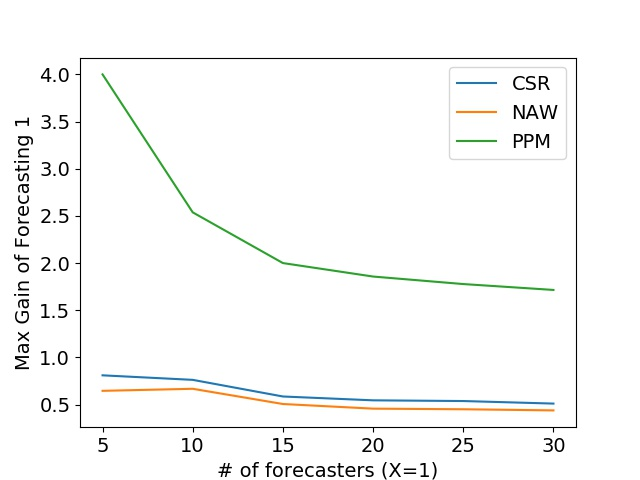
\includegraphics[width = \textwidth]{(UnifF_UnifW)Max_gain_of_forecasting_1.jpg}
        	\end{minipage}
        	\begin{minipage}{0.48\textwidth}
        	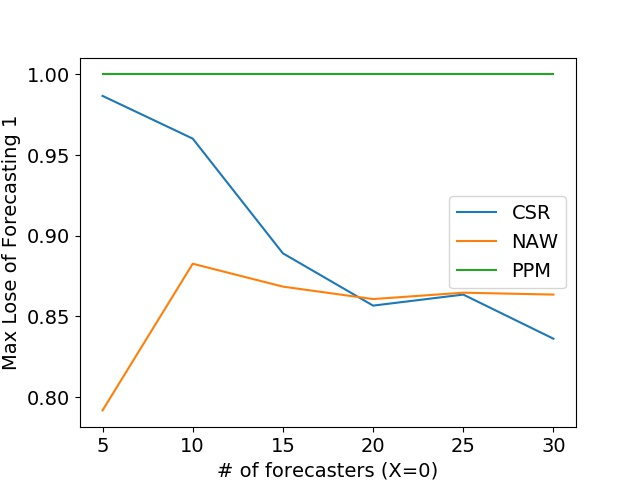
\includegraphics[width = \textwidth]{(UnifF_UnifW)Max_lose_of_forecasting_1.jpg}
        	\end{minipage}
        	\caption{The  extreme payoffs of forecasting 1 when others' are drawn from \textbf{uniform distribution}}
        	\end{figure}
	
	\begin{figure}[H]
        	\centering
        	\begin{minipage}{0.48\textwidth}
        	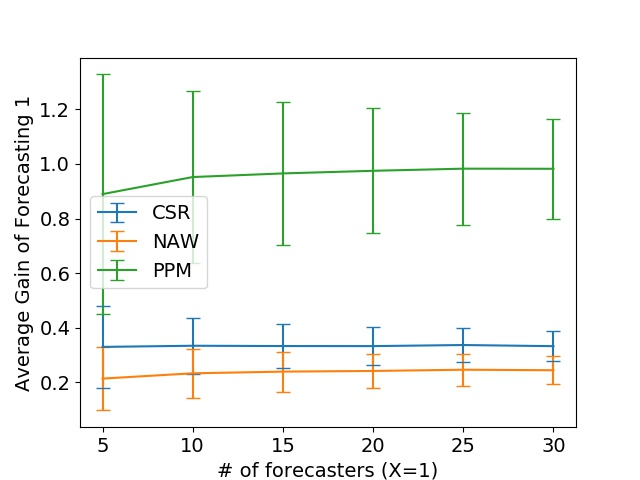
\includegraphics[width = \textwidth]{Ind(UnifF_UnifW)Avg_gain_of_forecasting_1.jpg}
        	\end{minipage}
        	\begin{minipage}{0.48\textwidth}
        	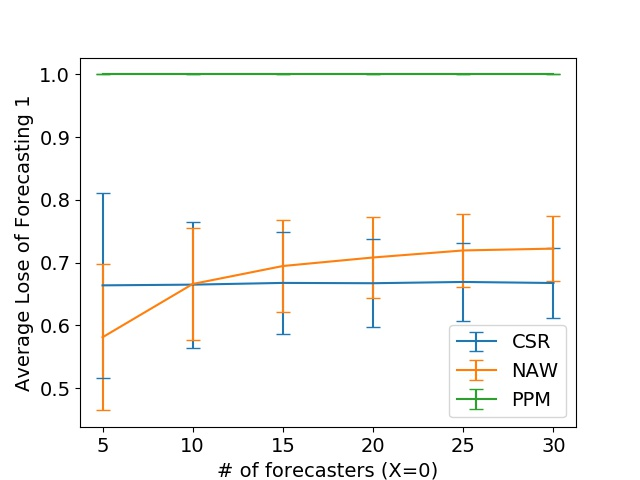
\includegraphics[width = \textwidth]{Ind(UnifF_UnifW)Avg_lose_of_forecasting_1.jpg}
        	\end{minipage}
        	\caption{The  average payoff of forecasting 1 when others' are drawn from \textbf{uniform distribution}}
        	\end{figure}
	
	\item The other forecasts follow Beta(1, 0.2), where the mode is forecasting 1.
	\begin{figure}[H]
        	\centering
        	\begin{minipage}{0.48\textwidth}
        	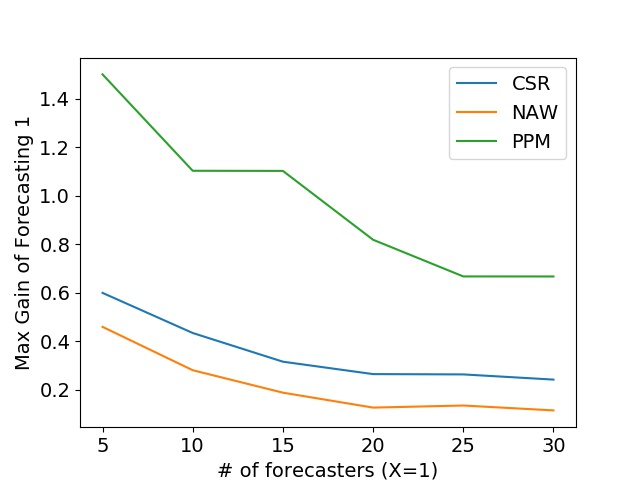
\includegraphics[width = \textwidth]{(Beta(1_0dot2)F_UnifW)Max_gain_of_forecasting_1.jpg}
        	\end{minipage}
        	\begin{minipage}{0.48\textwidth}
        	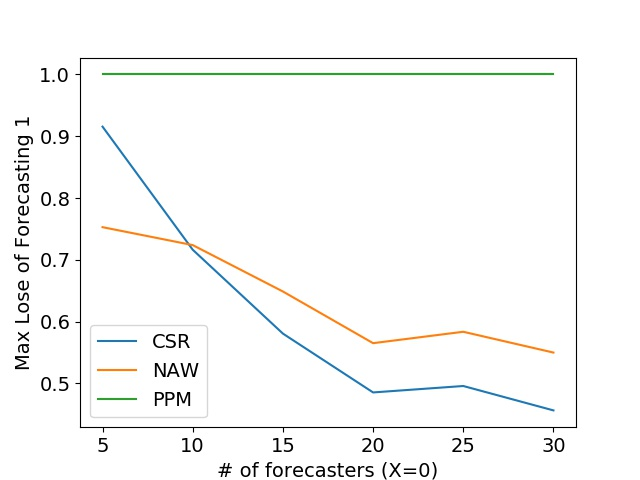
\includegraphics[width = \textwidth]{(Beta(1_0dot2)F_UnifW)Max_lose_of_forecasting_1.jpg}
        	\end{minipage}
        	\caption{The  extreme payoffs of forecasting 1 when others' are drawn from \textbf{Beta(1,0.2)}}
        	\end{figure}
	
	\begin{figure}[H]
        	\centering
        	\begin{minipage}{0.48\textwidth}
        	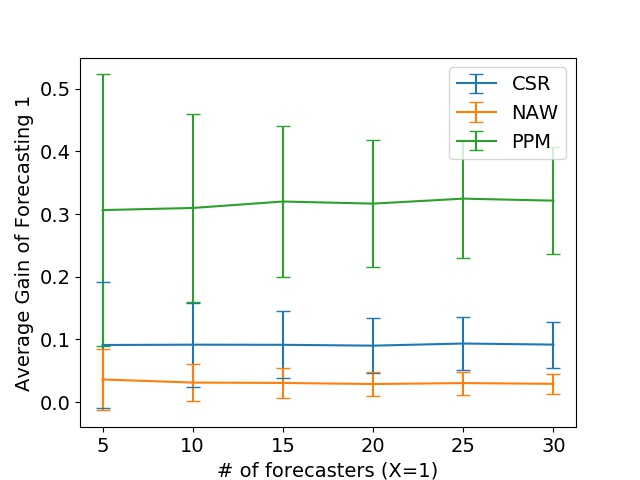
\includegraphics[width = \textwidth]{Ind(Beta(1_0dot2)F_UnifW)Avg_gain_of_forecasting_1.jpg}
        	\end{minipage}
        	\begin{minipage}{0.48\textwidth}
        	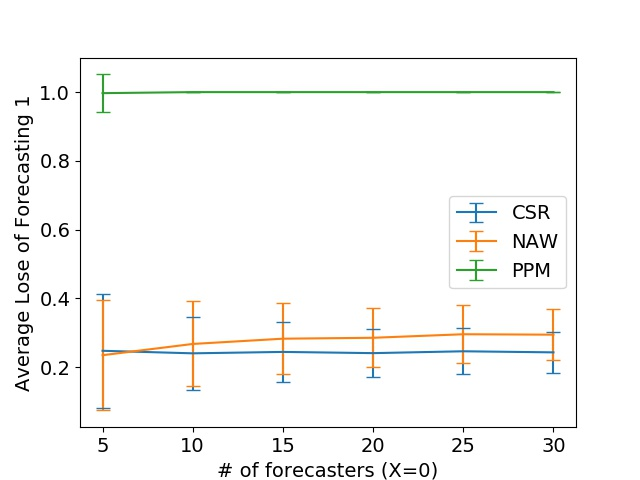
\includegraphics[width = \textwidth]{Ind(Beta(1_0dot2)F_UnifW)Avg_lose_of_forecasting_1.jpg}
        	\end{minipage}
        	\caption{The  average payoff of forecasting 1 when others' are drawn from \textbf{Beta(1,0.2)}}
        	\end{figure}
	
	\item The other forecasts follow Beta(0.2, 1), where the mode is forecasting 0.
	\begin{figure}[H]
        	\centering
        	\begin{minipage}{0.48\textwidth}
        	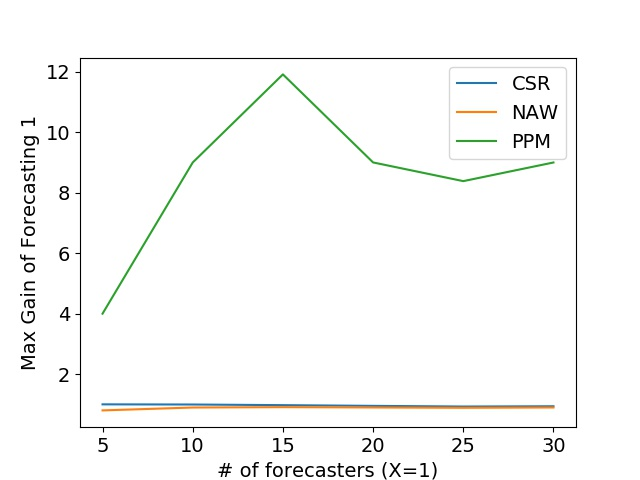
\includegraphics[width = \textwidth]{(Beta(0dot2_1)F_UnifW)Max_gain_of_forecasting_1.jpg}
        	\end{minipage}
        	\begin{minipage}{0.48\textwidth}
        	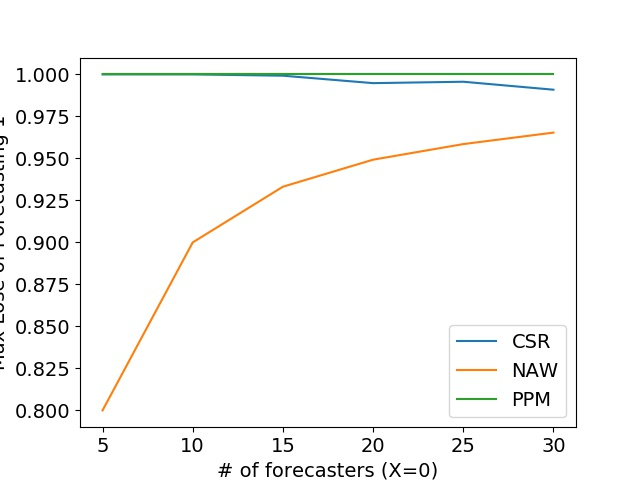
\includegraphics[width = \textwidth]{(Beta(0dot2_1)F_UnifW)Max_lose_of_forecasting_1.jpg}
        	\end{minipage}
        	\caption{The  extreme payoffs of forecasting 1 when others' are drawn from \textbf{Beta(0.2,1)}}
        	\end{figure}
	
	\begin{figure}[H]
        	\centering
        	\begin{minipage}{0.48\textwidth}
        	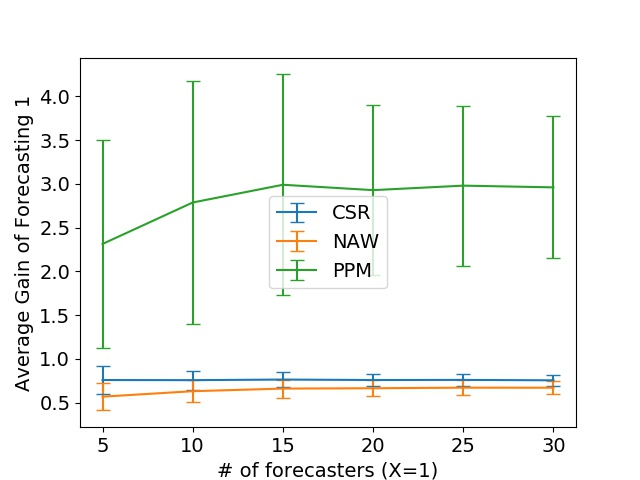
\includegraphics[width = \textwidth]{Ind(Beta(0dot2_1)F_UnifW)Avg_gain_of_forecasting_1.jpg}
        	\end{minipage}
        	\begin{minipage}{0.48\textwidth}
        	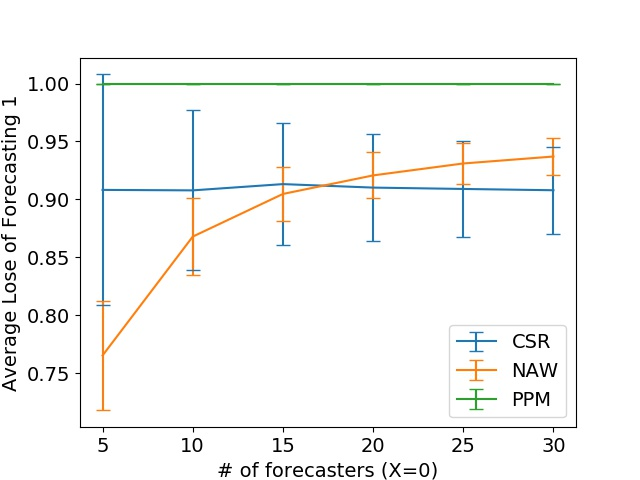
\includegraphics[width = \textwidth]{Ind(Beta(0dot2_1)F_UnifW)Avg_lose_of_forecasting_1.jpg}
        	\end{minipage}
        	\caption{The  average payoff of forecasting 1 when others' are drawn from \textbf{Beta(0.2,1)}}
        	\end{figure}
	
	\item The other forecasts follow Beta(100, 100), where the mode is forecasting 0.5.
	\begin{figure}[H]
        	\centering
        	\begin{minipage}{0.48\textwidth}
        	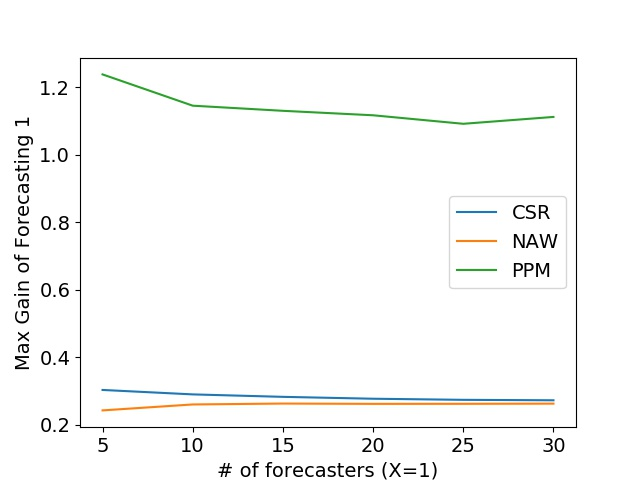
\includegraphics[width = \textwidth]{(Beta(100_100)F_UnifW)Max_gain_of_forecasting_1.jpg}
        	\end{minipage}
        	\begin{minipage}{0.48\textwidth}
        	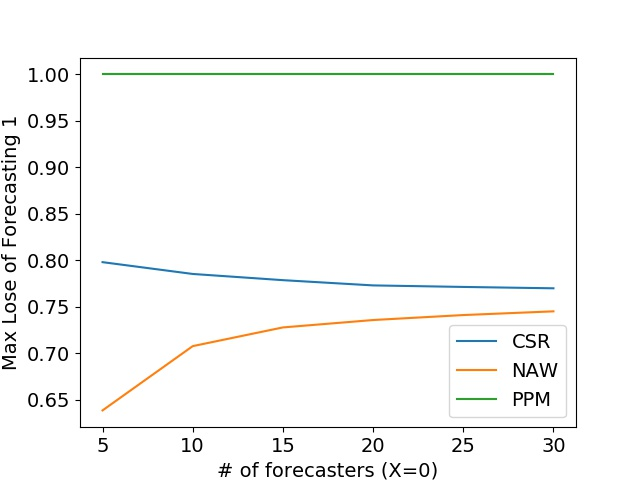
\includegraphics[width = \textwidth]{(Beta(100_100)F_UnifW)Max_lose_of_forecasting_1.jpg}
        	\end{minipage}
        	\caption{The  extreme payoffs of forecasting 1 when others' are drawn from \textbf{Beta(100,100)}}
        	\end{figure}
	
	\begin{figure}[H]
        	\centering
        	\begin{minipage}{0.48\textwidth}
        	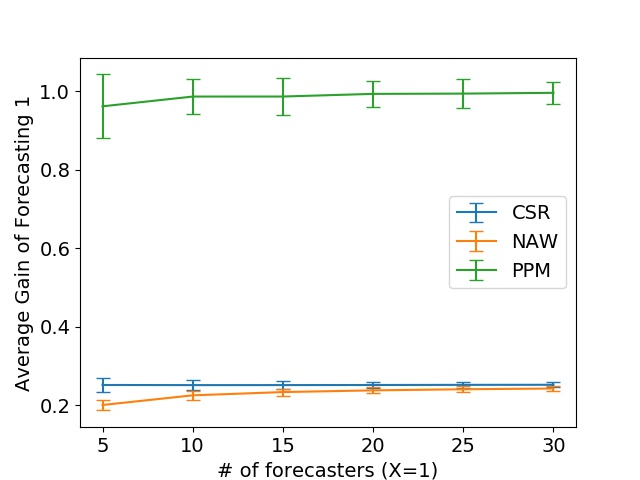
\includegraphics[width = \textwidth]{Ind(Beta(100_100)F_UnifW)Avg_gain_of_forecasting_1.jpg}
        	\end{minipage}
        	\begin{minipage}{0.48\textwidth}
        	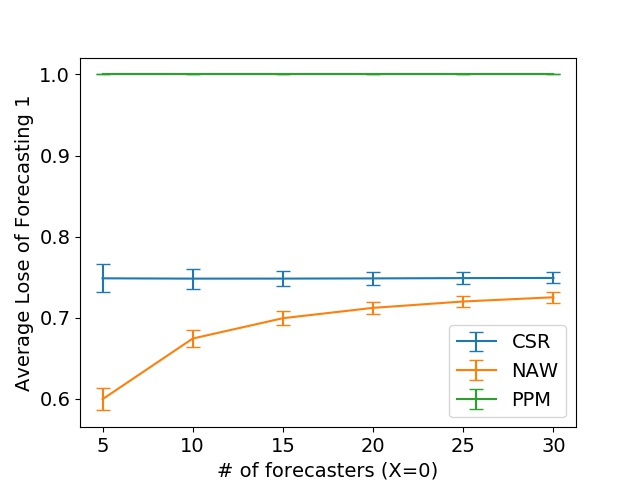
\includegraphics[width = \textwidth]{Ind(Beta(100_100)F_UnifW)Avg_lose_of_forecasting_1.jpg}
        	\end{minipage}
        	\caption{The average payoff of forecasting 1 when others' are drawn from \textbf{Beta(100,100)}}
        	\end{figure}
	\end{enumerate}

\subsection{Average performances of different mechanisms under different wager distributions}
	\begin{enumerate}
	\item Forecasts are drawn from uniform distribution, wagers are drawn from Beta(100,100) (normal-distribution-like with mean 0.5 in range [0,1])
	\begin{figure}[H]
        	\centering
        	\begin{minipage}{0.48\textwidth}
        	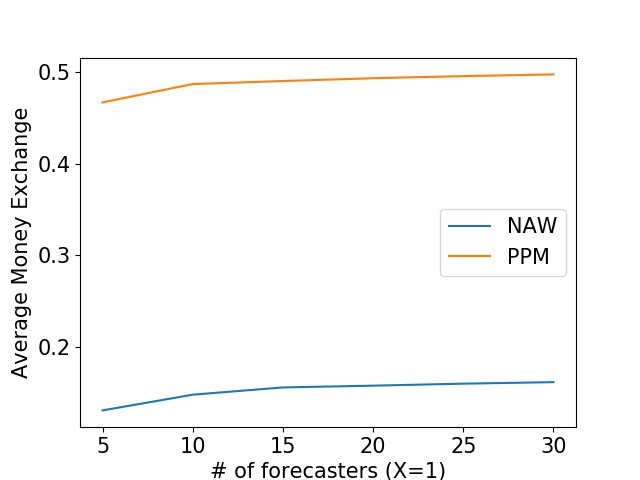
\includegraphics[width = \textwidth]{(UnifF_Beta(100_100)W)Avg_MnEx(X=1).jpg}
        	\end{minipage}
        	\begin{minipage}{0.48\textwidth}
        	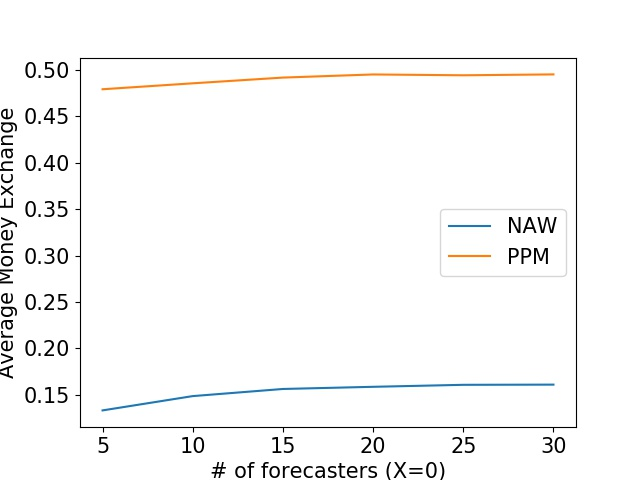
\includegraphics[width = \textwidth]{(UnifF_Beta(100_100)W)Avg_MnEx(X=0).jpg}
        	\end{minipage}
        	\caption{Average money exchange (Forecasts: Uniform, Wagers: Beta(100,100))}
        	\end{figure}
	
	\item Forecasts are drawn from uniform distribution, wagers are drawn from Pareto(1.16,1) ( in DCA paper)
	\begin{figure}[H]
        	\centering
        	\begin{minipage}{0.48\textwidth}
        	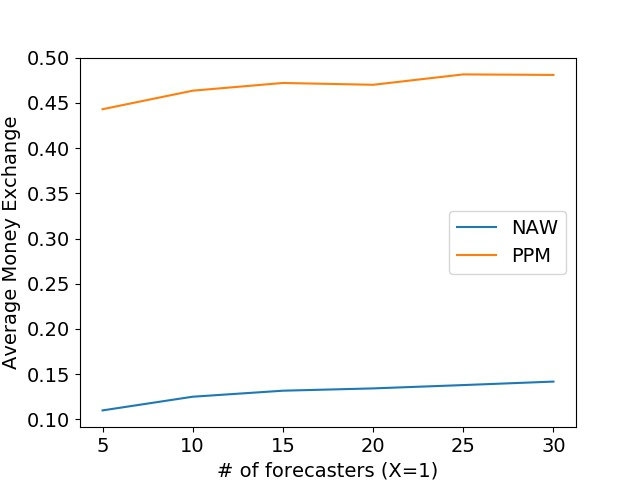
\includegraphics[width = \textwidth]{(UnifF_Pareto(1dot16_1)W)Avg_MnEx(X=1).jpg}
        	\end{minipage}
        	\begin{minipage}{0.48\textwidth}
        	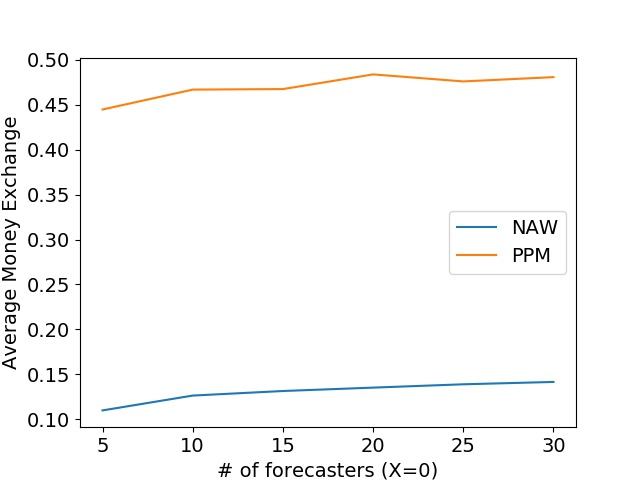
\includegraphics[width = \textwidth]{(UnifF_Pareto(1dot16_1)W)Avg_MnEx(X=0).jpg}
        	\end{minipage}
        	\caption{Average money exchange (Forecasts: \textbf{Uniform}, Wagers: \textbf{Pareto(1.16,1)})}
        	\end{figure}
	
	\item Forecasts are drawn from Beta(0.3,0.3), wagers are drawn from Beta(100,100) ( in DCA paper)
	\begin{figure}[H]
        	\centering
        	\begin{minipage}{0.48\textwidth}
        	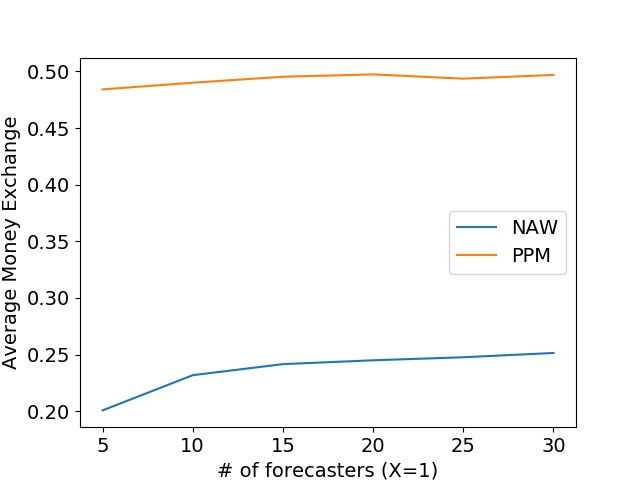
\includegraphics[width = \textwidth]{(Beta(0dot3_0dot3)F_Beta(100_100)W)Avg_MnEx(X=1).jpg}
        	\end{minipage}
        	\begin{minipage}{0.48\textwidth}
        	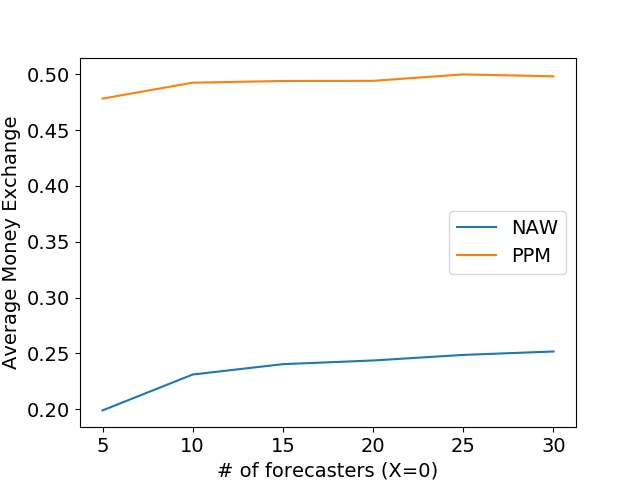
\includegraphics[width = \textwidth]{(Beta(0dot3_0dot3)F_Beta(100_100)W)Avg_MnEx(X=0).jpg}
        	\end{minipage}
        	\caption{Average money exchange (Forecasts: \textbf{Beta(0.3,0.3)}, Wagers: \textbf{Beta(100,100)})}
        	\end{figure}
	
	\item Forecasts are drawn from Beta(0.3,0.3), wagers are drawn from Pareto(1.16,1) ( in DCA paper)
	\begin{figure}[H]
        	\centering
        	\begin{minipage}{0.48\textwidth}
        	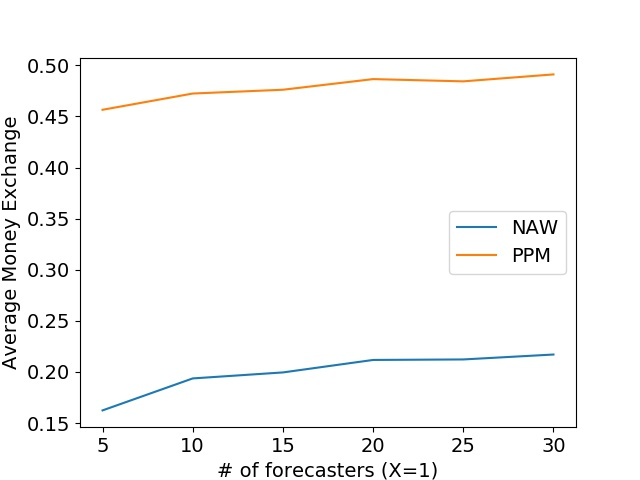
\includegraphics[width = \textwidth]{(Beta(0dot3_0dot3)F_Pareto(1dot16_1)W)Avg_MnEx(X=1).jpg}
        	\end{minipage}
        	\begin{minipage}{0.48\textwidth}
        	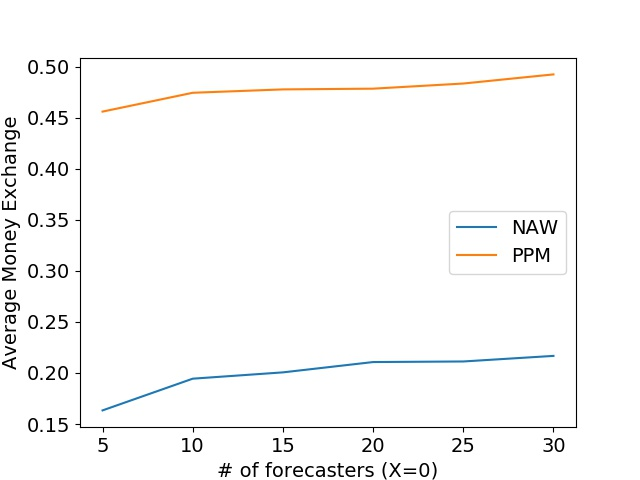
\includegraphics[width = \textwidth]{(Beta(0dot3_0dot3)F_Pareto(1dot16_1)W)Avg_MnEx(X=0).jpg}
        	\end{minipage}
        	\caption{Average money exchange (Forecasts: \textbf{Beta(0.3,0.3)}, Wagers: \textbf{Pareto(1.16,1)})}
        	\end{figure}
	
	
	
	\item Forecasts are drawn from Beta(1,0.2), wagers are drawn from Beta(100,100) (normal-distribution-like with mean 0.5 in range [0,1])

	\begin{figure}[H]
        	\centering
        	\begin{minipage}{0.48\textwidth}
        	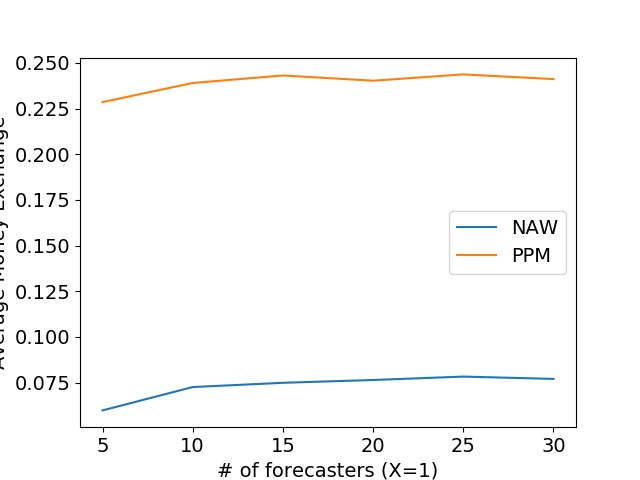
\includegraphics[width = \textwidth]{(Beta(1_0dot2)F_Beta(100_100)W)Avg_MnEx(X=1).jpg}
        	\end{minipage}
        	\begin{minipage}{0.48\textwidth}
        	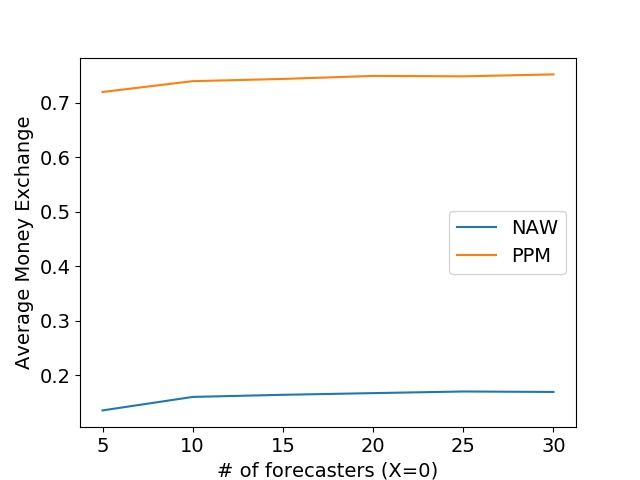
\includegraphics[width = \textwidth]{(Beta(1_0dot2)F_Beta(100_100)W)Avg_MnEx(X=0).jpg}
        	\end{minipage}
        	\caption{Average money exchange (Forecasts: \textbf{Beta(1,0.2)}, Wagers: \textbf{Beta(100,100)})}
        	\end{figure}
	
	
	
	\item Forecasts are drawn from Beta(1,0.2), wagers are drawn from Pareto(1.16,1) ( in DCA paper)
	\begin{figure}[H]
        	\centering
        	\begin{minipage}{0.48\textwidth}
        	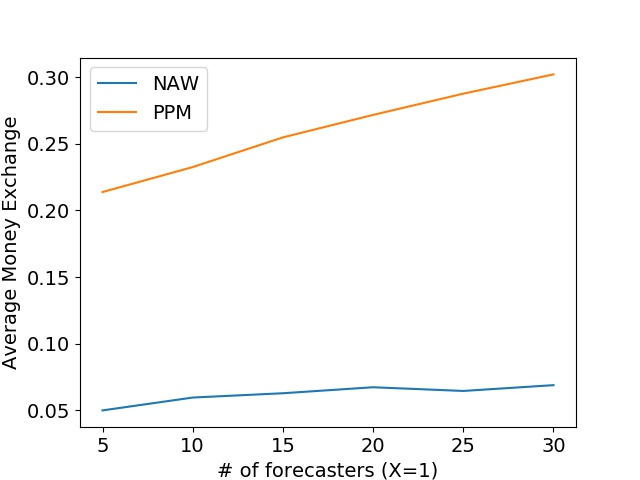
\includegraphics[width = \textwidth]{(Beta(1_0dot2)F_Pareto(1dot16_1)W)Avg_MnEx(X=1).jpg}
        	\end{minipage}
        	\begin{minipage}{0.48\textwidth}
        	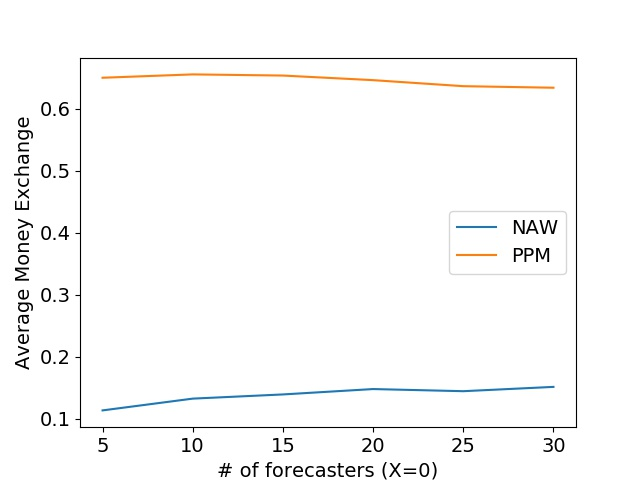
\includegraphics[width = \textwidth]{(Beta(1_0dot2)F_Pareto(1dot16_1)W)Avg_MnEx(X=0).jpg}
        	\end{minipage}
        	\caption{Average money exchange (Forecasts: \textbf{Beta(1,0.2)}, Wagers: \textbf{Pareto(1.16,1)})}
        	\end{figure}
	
	
	\end{enumerate}
	
\subsection{Average performances of different mechanisms with uniform wager}
	We ranged the number of forecasters for 5 to 50 with a step 5. For each number of forecasters, we ran 1000$\sim$10000 experiments. We recorded the average, maximum and minimum money exchange during these 10000 experiments.
	\begin{enumerate}
	\newpage
	\item Forecasts are generated by uniform distribution.
        	\begin{figure}[H]
        	\centering
        	\begin{minipage}{0.48\textwidth}
        %	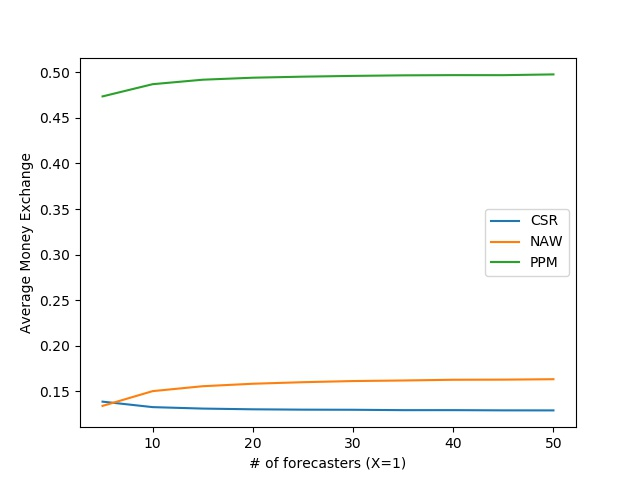
\includegraphics[width = \textwidth]{(uniform)Avg_MnEx(X=1).jpg}
        	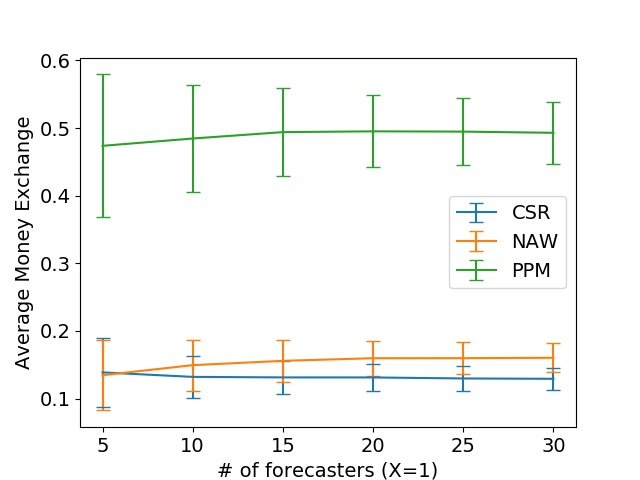
\includegraphics[width = \textwidth]{MnEx(UnifF_UnifW)Avg_MnEx(X=1).jpg}
        	\end{minipage}
        	\begin{minipage}{0.48\textwidth}
        %	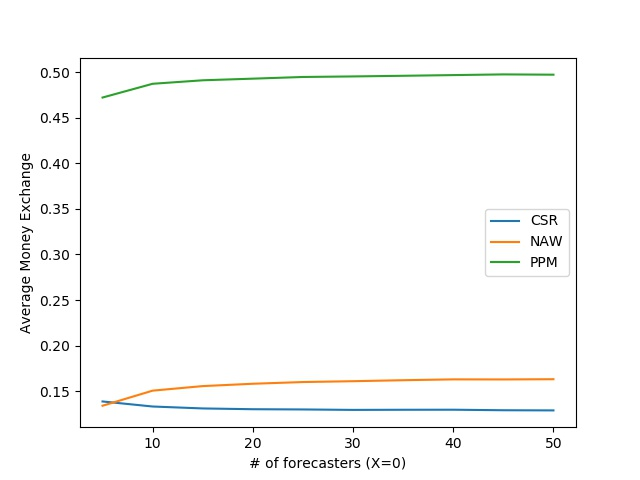
\includegraphics[width = \textwidth]{(uniform)Avg_MnEx(X=0).jpg}
        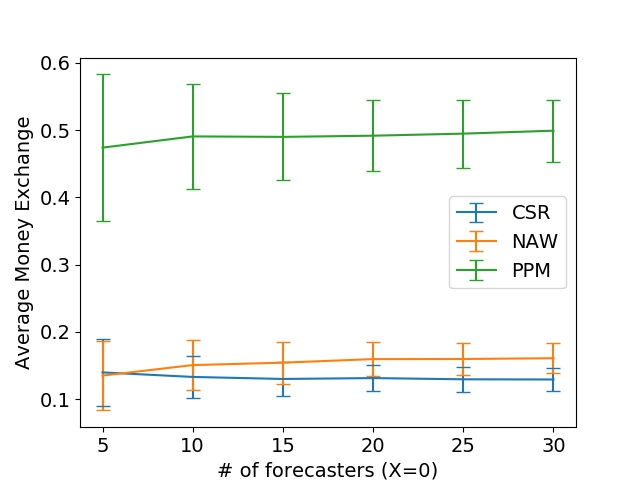
\includegraphics[width = \textwidth]{MnEx(UnifF_UnifW)Avg_MnEx(X=0).jpg}
        	\end{minipage}
        	\caption{Average money exchange over 1000 runs}
        	\end{figure}
        	
        	\begin{figure}[H]
        	\centering
        	\begin{minipage}{0.48\textwidth}
        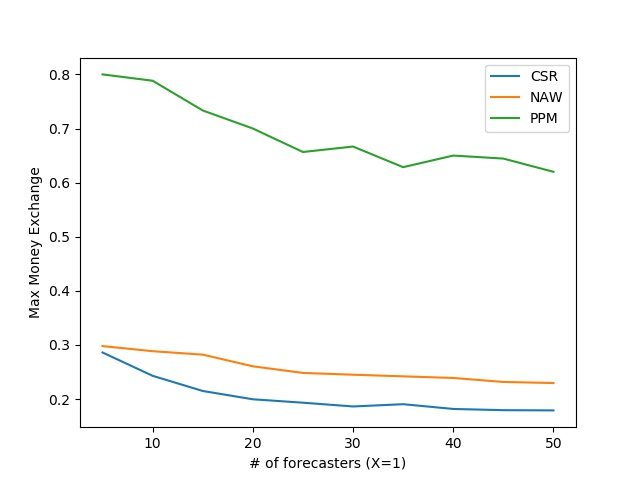
\includegraphics[width = \textwidth]{(uniform)Max_MnEx(X=1).jpg}
        	\end{minipage}
        	\begin{minipage}{0.48\textwidth}
        	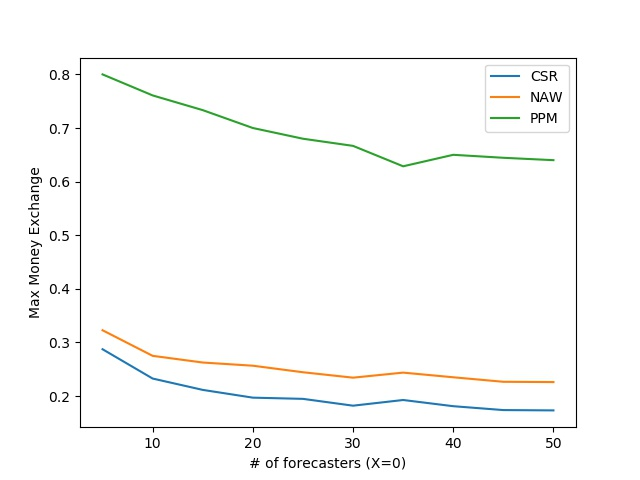
\includegraphics[width = \textwidth]{(uniform)Max_MnEx(X=0).jpg}
        	\end{minipage}
        	\caption{Maximum money exchange over 10000 runs}
        	\end{figure}
        	
        	\begin{figure}[H]
        	\centering
        	\begin{minipage}{0.48\textwidth}
        	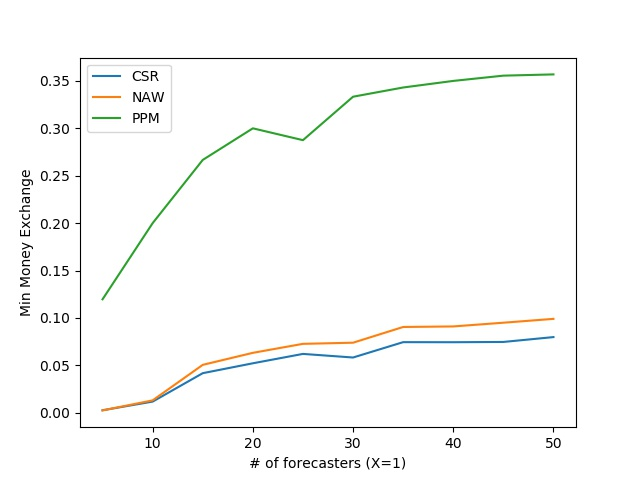
\includegraphics[width = \textwidth]{(uniform)Min_MnEx(X=1).jpg}
        	\end{minipage}
        	\begin{minipage}{0.48\textwidth}
        	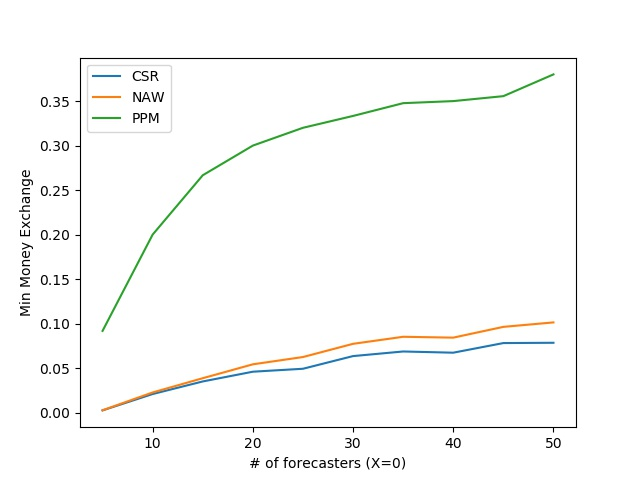
\includegraphics[width = \textwidth]{(uniform)Min_MnEx(X=0).jpg}
        	\end{minipage}
        	\caption{Minimum money exchange over 10000 runs}
        	\end{figure}
	
	\newpage
	\item Forecasts are generated by distribution $Beta(0.3, 0.3)$, which puts most probability mass on the two ends, i.e., $Pr(p>0.95)=0.23, Pr(p<0.05)=0.23$
	
        	\begin{figure}[H]
        	\centering
        	\begin{minipage}{0.48\textwidth}
        %	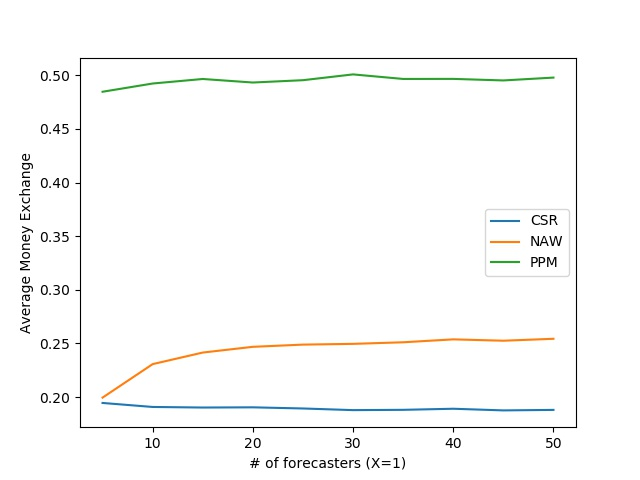
\includegraphics[width = \textwidth]{(Beta_0dot3_0dot3)Avg_MnEx(X=1).jpg}
        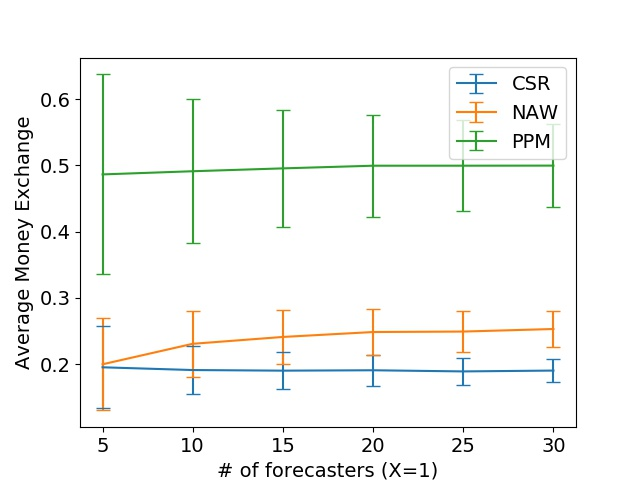
\includegraphics[width = \textwidth]{MnEx(Beta(0dot3_0dot3)F_UnifW)Avg_MnEx(X=1).jpg}
        	\end{minipage}
        	\begin{minipage}{0.48\textwidth}
        %	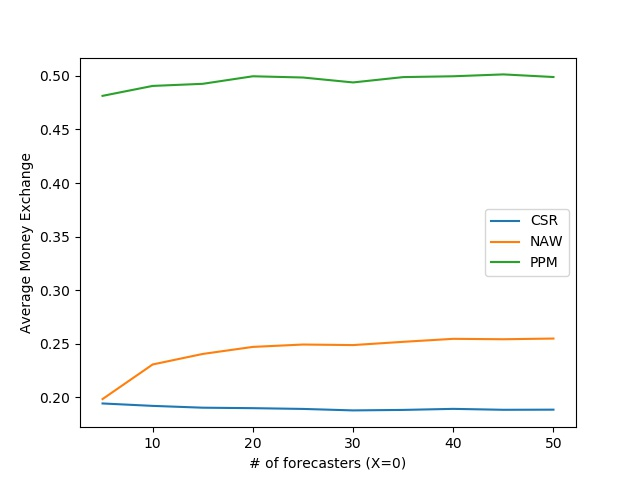
\includegraphics[width = \textwidth]{(Beta_0dot3_0dot3)Avg_MnEx(X=0).jpg}
        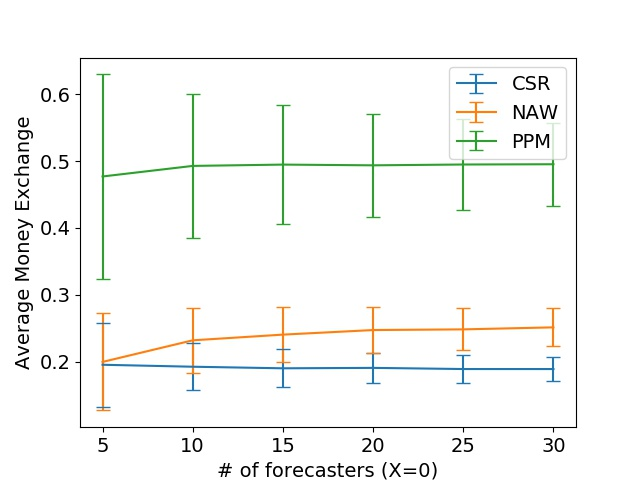
\includegraphics[width = \textwidth]{MnEx(Beta(0dot3_0dot3)F_UnifW)Avg_MnEx(X=0).jpg}
        	\end{minipage}
        	\caption{Average money exchange over 1000 runs}
        	\end{figure}
        	
        	\begin{figure}[H]
        	\centering
        	\begin{minipage}{0.48\textwidth}
        	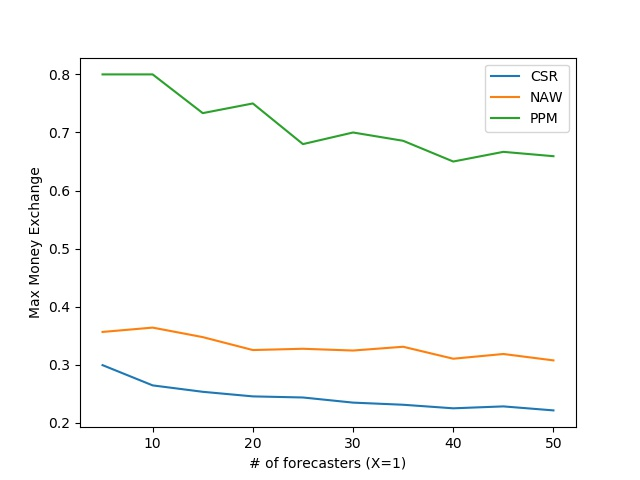
\includegraphics[width = \textwidth]{(Beta_0dot3_0dot3)Max_MnEx(X=1).jpg}
        	\end{minipage}
        	\begin{minipage}{0.48\textwidth}
        	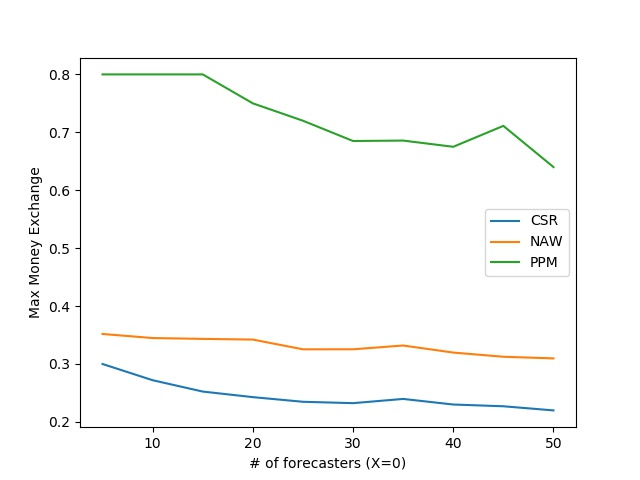
\includegraphics[width = \textwidth]{(Beta_0dot3_0dot3)Max_MnEx(X=0).jpg}
        	\end{minipage}
        	\caption{Maximum money exchange over 1000 runs}
        	\end{figure}
        	
        	\begin{figure}[H]
        	\centering
        	\begin{minipage}{0.48\textwidth}
        	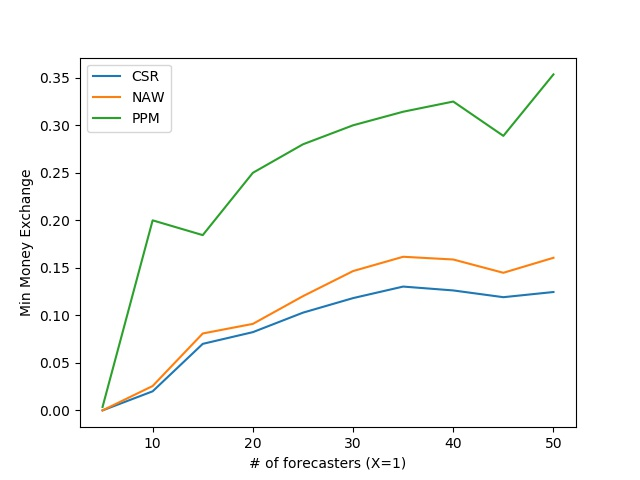
\includegraphics[width = \textwidth]{(Beta_0dot3_0dot3)Min_MnEx(X=1).jpg}
        	\end{minipage}
        	\begin{minipage}{0.48\textwidth}
        	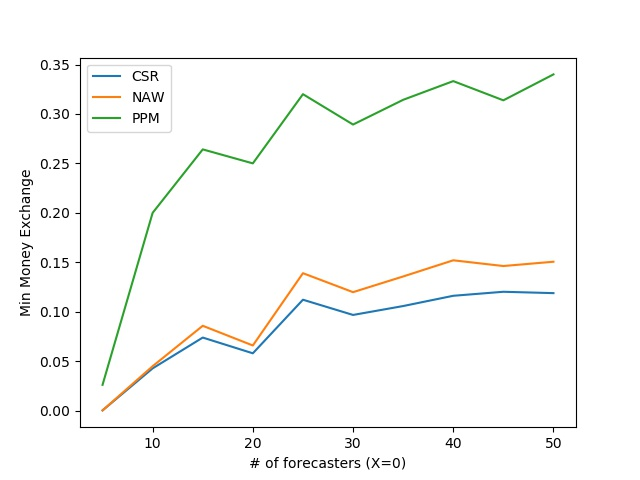
\includegraphics[width = \textwidth]{(Beta_0dot3_0dot3)Min_MnEx(X=0).jpg}
        	\end{minipage}
        	\caption{Minimum money exchange over 1000 runs}
        	\end{figure}
	
	\newpage
	\item Forecasts are generated by distribution $Beta(1, 0.2)$, which is a long-tail-like distribution over [0,1], i.e., $Pr(p>0.95)=0.55, Pr(p<0.5)=0.13, Pr(P<0.05)=0.01$.
	\begin{figure}[H]
        	\centering
        	\begin{minipage}{0.48\textwidth}
        %	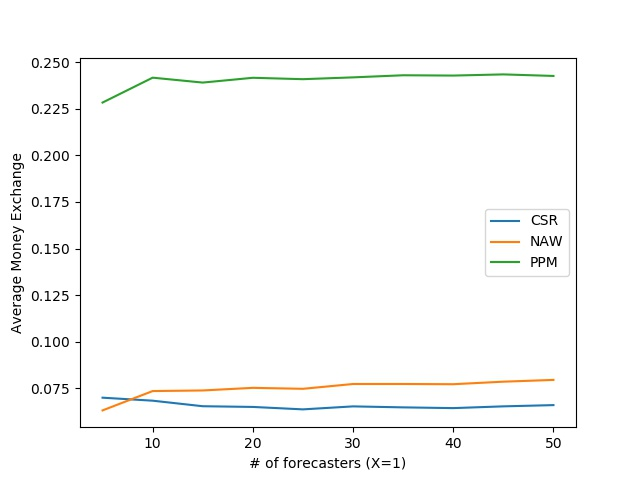
\includegraphics[width = \textwidth]{(Beta_1_0dot2)Avg_MnEx(X=1).jpg}
        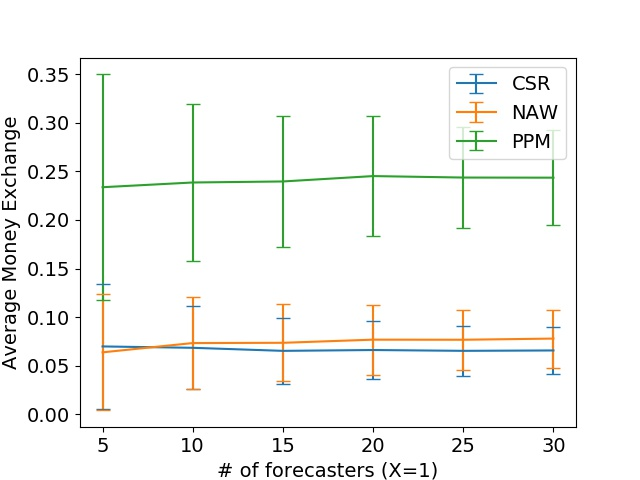
\includegraphics[width = \textwidth]{MnEx(Beta(1_0dot2)F_UnifW)Avg_MnEx(X=1).jpg}
        	\end{minipage}
        	\begin{minipage}{0.48\textwidth}
        %	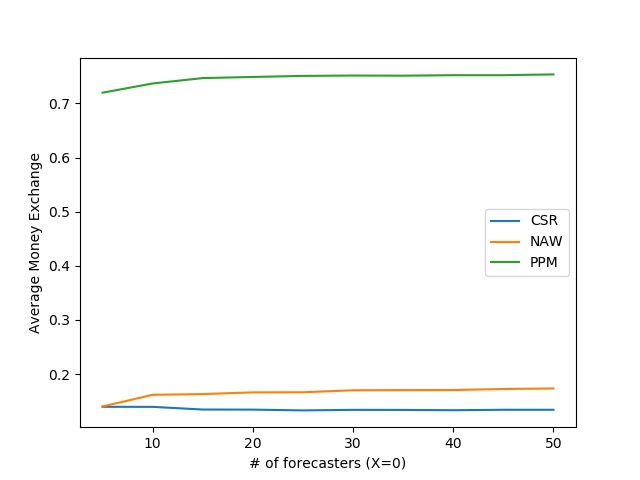
\includegraphics[width = \textwidth]{(Beta_1_0dot2)Avg_MnEx(X=0).jpg}
        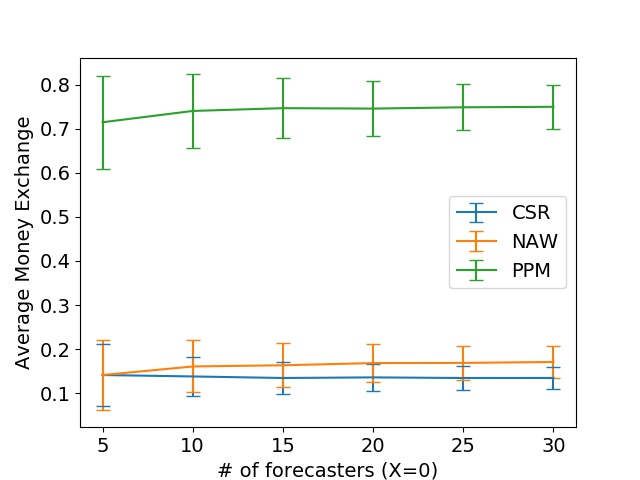
\includegraphics[width = \textwidth]{MnEx(Beta(1_0dot2)F_UnifW)Avg_MnEx(X=0).jpg}
        	\end{minipage}
        	\caption{Average money exchange over 1000 runs}
        	\end{figure}
        	
        	\begin{figure}[H]
        	\centering
        	\begin{minipage}{0.48\textwidth}
        	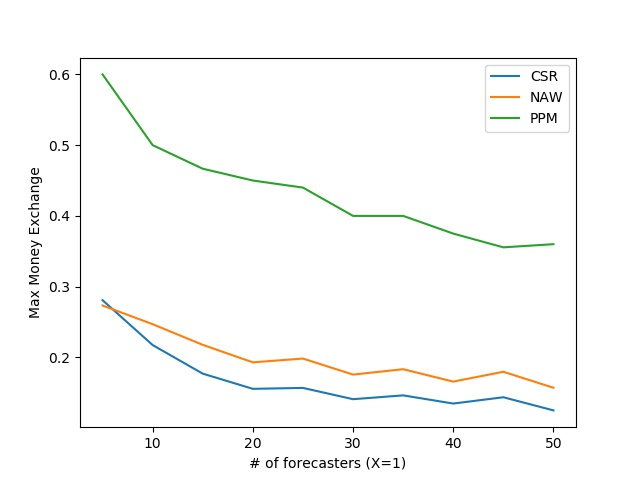
\includegraphics[width = \textwidth]{(Beta_1_0dot2)Max_MnEx(X=1).jpg}
        	\end{minipage}
        	\begin{minipage}{0.48\textwidth}
        	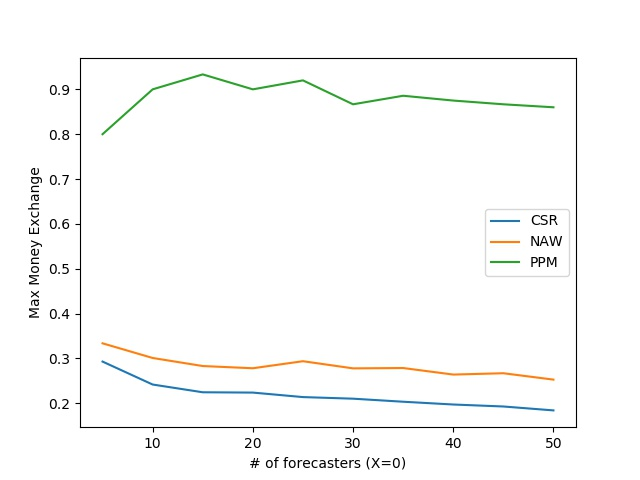
\includegraphics[width = \textwidth]{(Beta_1_0dot2)Max_MnEx(X=0).jpg}
        	\end{minipage}
        	\caption{Maximum money exchange over 1000 runs}
        	\end{figure}
        	
        	\begin{figure}[H]
        	\centering
        	\begin{minipage}{0.48\textwidth}
        	\includegraphics[width = \textwidth]{(Beta_1_0dot2)Min_MnEx(X=1).jpg}
        	\end{minipage}
        	\begin{minipage}{0.48\textwidth}
        	\includegraphics[width = \textwidth]{(Beta_1_0dot2)Min_MnEx(X=0).jpg}
        	\end{minipage}
        	\caption{Minimum money exchange over 1000 runs}
        	\end{figure}
	
	\newpage
	\item Forecasts are generated by distribution $Beta(100, 100)$, which is a normal-distribution-like distribution, putting all probability mass over [0.35,0.65] with expectation 0.5.
		\begin{figure}[H]
        	\centering
        	\begin{minipage}{0.48\textwidth}
%        	\includegraphics[width = \textwidth]{(Beta_100_100)Avg_MnEx(X=1).jpg}
        \includegraphics[width = \textwidth]{MnEx(Beta(100_100)F_UnifW)Avg_MnEx(X=1).jpg}
        	\end{minipage}
        	\begin{minipage}{0.48\textwidth}
%        	\includegraphics[width = \textwidth]{(Beta_100_100)Avg_MnEx(X=0).jpg}
        \includegraphics[width = \textwidth]{MnEx(Beta(100_100)F_UnifW)Avg_MnEx(X=0).jpg}
        	\end{minipage}
        	\caption{Average money exchange over 1000 runs}
        	\end{figure}
        	
        	\begin{figure}[H]
        	\centering
        	\begin{minipage}{0.48\textwidth}
        	\includegraphics[width = \textwidth]{(Beta_100_100)Max_MnEx(X=1).jpg}
        	\end{minipage}
        	\begin{minipage}{0.48\textwidth}
        	\includegraphics[width = \textwidth]{(Beta_100_100)Max_MnEx(X=0).jpg}
        	\end{minipage}
        	\caption{Maximum money exchange over 1000 runs}
        	\end{figure}
        	
        	\begin{figure}[H]
        	\centering
        	\begin{minipage}{0.48\textwidth}
        	\includegraphics[width = \textwidth]{(Beta_100_100)Min_MnEx(X=1).jpg}
        	\end{minipage}
        	\begin{minipage}{0.48\textwidth}
        	\includegraphics[width = \textwidth]{(Beta_100_100)Min_MnEx(X=0).jpg}
        	\end{minipage}
        	\caption{Minimum money exchange over 1000 runs}
        	\end{figure}
	\end{enumerate}

\end{document}